%% 
%% Copyright 2007-2020 Elsevier Ltd
%% 
%% This file is part of the 'Elsarticle Bundle'.
%% ---------------------------------------------
%% 
%% It may be distributed under the conditions of the LaTeX Project Public
%% License, either version 1.2 of this license or (at your option) any
%% later version.  The latest version of this license is in
%%    http://www.latex-project.org/lppl.txt
%% and version 1.2 or later is part of all distributions of LaTeX
%% version 1999/12/01 or later.
%% 
%% The list of all files belonging to the 'Elsarticle Bundle' is
%% given in the file `manifest.txt'.
%% 
%% Template article for Elsevier's document class `elsarticle'
%% with harvard style bibliographic references

\documentclass[review,12pt,authoryear]{elsarticle}

%% Use the option review to obtain double line spacing
%% \documentclass[authoryear,preprint,review,12pt]{elsarticle}

%% Use the options 1p,twocolumn; 3p; 3p,twocolumn; 5p; or 5p,twocolumn
%% for a journal layout:
%% \documentclass[final,1p,times,authoryear]{elsarticle}
%% \documentclass[final,1p,times,twocolumn,authoryear]{elsarticle}
%% \documentclass[final,3p,times,authoryear]{elsarticle}
%% \documentclass[final,3p,times,twocolumn,authoryear]{elsarticle}
%% \documentclass[final,5p,times,authoryear]{elsarticle}
%% \documentclass[final,5p,times,twocolumn,authoryear]{elsarticle}

%% For including figures, graphicx.sty has been loaded in
%% elsarticle.cls. If you prefer to use the old commands
%% please give \usepackage{epsfig}

%% The amssymb package provides various useful mathematical symbols
\usepackage{amssymb}
%% The amsthm package provides extended theorem environments
%% \usepackage{amsthm}

%% The lineno packages adds line numbers. Start line numbering with
%% \begin{linenumbers}, end it with \end{linenumbers}. Or switch it on
%% for the whole article with \linenumbers.
\usepackage{lineno}

\journal{Geography and Sustainability}

\begin{document}
\begin{linenumbers}
\begin{frontmatter}


%% Title, authors and addresses

%% use the tnoteref command within \title for footnotes;
%% use the tnotetext command for theassociated footnote;
%% use the fnref command within \author or \affiliation for footnotes;
%% use the fntext command for theassociated footnote;
%% use the corref command within \author for corresponding author footnotes;
%% use the cortext command for theassociated footnote;
%% use the ead command for the email address,
%% and the form \ead[url] for the home page:
%% \title{Title\tnoteref{label1}}
%% \tnotetext[label1]{}
%% \author{Name\corref{cor1}\fnref{label2}}
%% \ead{email address}
%% \ead[url]{home page}
%% \fntext[label2]{}
%% \cortext[cor1]{}
%% \affiliation{organization={},
%%            addressline={}, 
%%            city={},
%%            postcode={}, 
%%            state={},
%%            country={}}
%% \fntext[label3]{}

    \title{Resource Use and the Value-Productivity Tradeoff in Australian Winegrowing Regions}


%% use optional labels to link authors explicitly to addresses:
%% \author[label1,label2]{}
%% \affiliation[label1]{organization={},
%%             addressline={},
%%             city={},
%%             postcode={},
%%             state={},
%%             country={}}
%%
%% \affiliation[label2]{organization={},
%%             addressline={},
%%             city={},
%%             postcode={},
%%             state={},
%%             country={}}

    \affiliation[label1]{organization={QUT},
                 addressline={},
                 city={},
                 postcode={},
                 state={QLD},
                 country={}}
    \affiliation[label2]{organization={AWRI},
                 addressline={},
                 city={},
                 postcode={},
                 state={SA},
                 country={}}
    \affiliation[label3]{organization={Food Agility CRC},
                 addressline={},
                 city={},
                 postcode={},
                 state={Vic},
                 country={}}
\author[label1,label2,label3]{Bryce Polley}
\date{20/06/2023}

      


    \begin{abstract}
      %% Text of abstract
      Lorem ipsum dolor sit amet, consectetur adipiscing elit, sed do eiusmod tempor incididunt ut labore et dolore magna aliqua. Ut enim ad minim veniam, quis nostrud exercitation ullamco laboris nisi ut aliquip ex ea commodo consequat. Duis aute irure dolor in reprehenderit in voluptate velit esse cillum dolore eu fugiat nulla pariatur. Excepteur sint occaecat cupidatat non proident, sunt in culpa qui officia deserunt mollit anim id est laborum.
      \end{abstract}

      %%Graphical abstract
      \begin{graphicalabstract}
        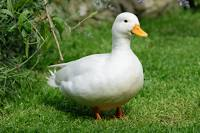
\includegraphics{graphical_abstract.jpeg}
      \end{graphicalabstract}

      \begin{keyword}
      %% keywords here, in the form: keyword \sep keyword
      keyword one \sep keyword two
      %% PACS codes here, in the form: \PACS code \sep code
      \PACS 0000 \sep 1111
      %% MSC codes here, in the form: \MSC code \sep code
      %% or \MSC[2008] code \sep code (2000 is the default)
      \MSC 0000 \sep 1111
      \end{keyword}
      

      %%Research highlights
      \begin{highlights}
        \item Research highlight 1
        \item Research highlight 2
        \end{highlights}

      \end{frontmatter}

%%%%%%%%%%%%%%%%%%%%%%%%%%%%%%%%%%%%%%%%%%
%%                main text             %%
%%%%%%%%%%%%%%%%%%%%%%%%%%%%%%%%%%%%%%%%%%

\section{Introduction}
The global focus on sustainability in agronomic industries has changed the way in which these enterprises do business. When strategies for a sustainable winegrowing industry are assessed, there is a trade-off between balancing the amount of resources invested and the resultant yield verses quality produced. This dilemma exists across agriculture within shared fundamental considerations such as water and nitrogen inputs \citep{hemmingCherryTomatoProduction2020,kawasakiQualityMattersMore2016, zhuEffectsNitrogenLevel2017}. Within viticulture (the cultivation of grapes for wine production) quality is driven by its integration within the wine industry; with a wine's potential quality being initially defined through the chemical makeup of the grapes used in its production. The consideration of sustainability is further complicated by environmental and socio-demographic pressures. In the Australian context, these include biosecurity, climate and international market demands.
\newline
In this analysis we observe relationships between yield and quality through the use of linear models. Quality can be defined in a variety of ways, for example analysing grapes' aroma, chemical composition and color. For the purpose of this study, quality was defined by winegrape crops' financial value per tonne. This definition assumes due diligence on the side of those that purchased the grapes; where market value of grapes heavily relies on grape quality \citep{yeggeInfluenceSensoryNonsensory2001}. Wine Australia also links grape quality to price per tonne, by explicitly defining grape quality within discrete price brackets.
\newline
An extensive amount of research into a variety of factors' effect on grape quality and yield exists.
% there needs to be references if there is extensive research
Due to the lack of long-term and in-depth data, individual effects are often studied in isolation \citep{abbalDecisionSupportSystem2016}. The lack of consolidated datasets also restricts the ability to gain statistical insights at large scales and across multiple regions \citep{keithjonesAustralianWineIndustry2002,knightFirmResourcesDevelopment2019}. The dataset used for this analysis includes data collected for the past 10 years from a multitude of vineyards located over a diverse range of Australian winegrowing regions.
\newline
We aim to use this broad dataset to confirm the existence of a yield verse quality trade off within Australian winegrowing; one not prior confirmed explicitly across such extensive diversities.
% you require a reference here
In achieving this, the context of how resource use relates to yield and quality will also be described. We link these relations to the potential for improvement through decision-making processes, and highlight that the way moving forward will require the optimisation of this process. The practical addition of these aims is a baseline for comparison - given a vineyard within Australia, one could extrapolate their comparative efficiency with regard to the tradeoff between invested resources, yield and quality.
\section{Methods}
We created four linear models to explore relationships between resources used and vineyard outputs (see Table 1). The response variables of the models were yield and quality, with yield being measured in tonnes and quality being the product of yield and the average sale price per tonne. Both response variables were examined as totals and as scales of area harvested. Values were compared in this manner to observe how economies of scale affect the use of resources.

\begin{table}[]
    \begin{center}
      \caption{Summary of models; their predictors, covariates and variable interactions.}
      \label{tab:tab1}
      \begin{tabular}{ccccc}
        & Response & Predictors & Covariates & Interactions \\
        Model 1 & Yield & Water Used, Scope 1 Emissions & Area Harvested, Year, GI Region & N\textbackslash A \\
        Model 2 & ${ \textrm{Yield}}\over{ \textrm{Area Harvested}}$ & Water Used, Scope 1 Emissions & Area Harvested, Year, GI Region & Area Harvested * Scope 1 Emissions, Area Harvested * Water Use, Year * Region \\
        Model 3 & \small{$\textrm{Yield} {\times} \textrm{Average Sale Price}$} &  Water Used, Scope 1 Emissions& Area Harvested, Year, GI Region & Area Harvested * Scope 1 Emissions, Area Harvested * Water Use, Year * Region  \\
        Model 4 & ${\textrm{Yield} \times \textrm{Average Sale Price}}\over{\textrm{Area Harvested}}$ & Water Used, Scope 1 Emissions & Area Harvested, Year, GI Region  & N\textbackslash A
      \end{tabular}
    \end{center}
\end{table}

\subsection{Data}
Data used in this analysis was provided by Sustainable Winegrowing Australia, Australia's national wine industry sustainability program; which aims to facilitate grape-growers and winemakers in demonstrating and improving their sustainability \citep{swaSustainableWingrowingAustralia2022}. Data recorded by Sustainable Winegrowing Australia is entered manually by winegrowers using a web based interface, with some fields being optional. Two subsets of this data were defined through vineyards which did not record average price of sale per tonne, and vineyards which did or which were in a region of known average price. Vineyards which did not record a value for average price of sale per tonne but were within regions with a recorded average price of sale per tonne by Wine Australia were filled in using this regional average. Both subsets contained: region, harvest year, yield, area harvested, water used and fuel used (diesel, petrol, biodiesel and LPG). To enable comparisons, total fuel was converted to equivalent carbon emissions in metric tons. 

The first subset of data was used for Model 1 and Model 2 (see Table 1). This subset contained 5298 samples spanning the period from 2012 to 2022, covering 57 GI Regions and 1432 separate vineyards.

The second subset of data, was limited to vineyards that recorded a value for their average sale price of grapes per tonne. This subset was used for Model 3 and Model 4 (see Table 1); and contained 2878 samples spanning the period from 2015 to 2022, covering 51 GI Regions and 944 separate vineyards.

Data was limited to samples that had recorded values for variables used (see Table 1). After reviewing correlation coefficients the data was logarithmically transformed, centred and scaled by standard deviation. Two values for average sale price were removed from the dataset, due to a recording of \$1. 
% \citep{wineaustraliaNationalVintageReport2019,wineaustraliaNationalVintageReport2020,wineaustraliaNationalVintageReport2021,wineaustraliaNationalVintageReport2022,winemakersfederationofaustraliaNationalVintageReport2012,winemakersfederationofaustraliaNationalVintageReport2013,winemakersfederationofaustraliaNationalVintageReport2014,winemakersfederationofaustraliaNationalVintageReport2015,winemakersfederationofaustraliaNationalVintageReport2016,winemakersfederationofaustraliaNationalVintageReport2017,winemakersfederationofaustraliaNationalVintageReport2018}.

Other variables including the use of renewable energy, contractors; and pressures such as frost, fire and disease were also explored. Variables that did not significantly contribute to the prediction of a response variable were excluded.

\subsection{Total Emissions}
Emissions were calculated from the total diesel, petrol, bio-diesel and LPG used for irrigation and activities within the vineyard. The equations given from the Australian National Greenhouse Accounts Factors, shown as 

\begin{equation}
\label{(1)}
    tCO_{2}e={{Q \times EC \times EF1 + EF3}\over{1000}},
\end{equation}

was used to convert the quantity of fuel in litres, $Q$, using a prescribed Energy Content, $EC$, and emission factors of scope one, $EF1$, and scope three, $EF3$, to tonnes of Carbon Dioxide equivalent, $tCO2e$ \citep{departmentofclimatechangeenergytheenvironmentandwaterAustralianNationalGreenhouse2022}.

The variables were reviewed for correlations by using a Pearson's Correlation Coefficient (see Tables 1, 2 and 3). This was undertaken for data on the original scale (see Table 1) and for data as a logarithmic transform (see Table 2). All P-values were found to be significant (< 2.200E-16), except the non-transformed values for water used (see Table 3). The logarithmic transforms performed the best due to a skew likely caused by a greater number of smaller vineyards within the dataset (see Table 4).

\subsection{Region}
The site of a vineyard predetermines several physical parameters such as climate, geology and soil; making location a widely considered key determinant of grape yield and quality \citep{abbalDecisionSupportSystem2016,agostaRegionalClimateVariability2012,fragaMultivariateClusteringViticultural2017}. Differences in vineyard locations were captured through the use of Geographical Indicator Regions (GI Regions). Each GI Region has its own unique mixture of climatic and geophsical properties that describes a unique winegrowing region within Australia; these regions were predefined by Wine Australia \citep{hallidayAustralianWineEncyclopedia2009,oliverReviewSoilPhysical2013,soarClimateDriversRed2008}.

The climatic properties of a GI Region are summarised in the Sustainable Winegrowing Australia user manual \citep{swaSustainableWinegrowingAustralia2021}. The user manual describes climates by rainfall and temperature, creating supersets of Regions of similar climatic properties. The climatic groups were used to illustrate similarities and differences occurring in areas larger than GI regions.

\subsection{Analysis}
General Linear Models were used as they offered the ability to produce statistical models that were explicit in the relationships between predictors and response variables. They also allowed the exploration of interactions between predictors and easily comparable differences in the influence and magnitude of relationships.

Data preprocessing, such as logarithmic transforms, was done using the Python programming language \citep{g.vanrossumPythonTutorialTechnical1995}. Linear models were created using the R statistical programming language \citep{rcoreteamLanguageEnvironmentStatistical2021}. These models were created iteratively to explore a variety of variable interactions and approaches to modelling the data. Not all explored approaches yielded improvements or accurate models. Alternate approaches included the use of Splines, hierarchical regression, Additive and Generalised Linear Models. Other variables were also explored but not used due to low reporting values such as fertiliser, tractor and contractor use. The use of only scope one emissions was due to the same reason where scope 2 sources were recorded sporadically at best.

\subsection{Model Validation}
Models were validated using K-fold cross validation calculated through the R Caret Package \citep{kuhnBuildingPredictiveModels2008}. K-fold cross validation works by removing a subset of data from the sample used to train models and then predicts those variables to determine how sensitive the model is to changes in the sample data. For this analysis each model was validated using 10 folds, repeated 100 times. % A reference for this is absolutely needed.

\section{Results}
\subsection{Exploratory Analysis}
Simple linear relationships between variables were explored using Pearson Correlation Coefficients. This was undertaken for data on the original scale (see Table 2) and for data as a logarithmic transform (see Table 3). Strong relationships were found to be present, as all P-values were considered significant (< 2.200E-16, see Tables 2 and 3), except for the non-transformed values for water used (see Table 4). The logarithmic transforms showed the strongest correlations, this was likely due to a skew caused by a greater number of smaller vineyards within the dataset (see Table 5).

\begin{table}[]
  \caption{Summary of models, their predictors, covariates and variable interactions.}
  \label{tab:tab2}
  \begin{tabular}{cccccccc}
  Variable                             & Yield      & Area       & Water Used & Scope One Emissions & $\textrm{Yield}\over\textrm{Area}$ & Average Price Per Tonne & ${\textrm{Average Price per tonne}\over\textrm{Area}}$ \\
  Yield                                & 1.000E+00  & 7.440E-01  & -4.309E-03 & 7.290E-01           & 3.500E-01            & -2.262E-01              & -1.644E-01                           \\
  Area                                 & 7.440E-01  & 1.000E+00  & -5.331E-03 & 8.921E-01           & 7.854E-02            & -1.178E-01              & -2.042E-01                           \\
  Water Used                           & -4.309E-03 & -5.331E-03 & 1.000E+00  & -1.929E-03          & -5.600E-03           & -3.562E-02              & -2.669E-02                           \\
  Scope One Emissions                  & 7.290E-01  & 8.921E-01  & -1.929E-03 & 1.000E+00           & 9.357E-02            & -9.422E-02              & -1.933E-01                           \\
  $\textrm{Yield}\over\textrm{Area}$                 & 3.500E-01  & 7.854E-02  & -5.600E-03 & 9.357E-02           & 1.000E+00            & -4.849E-01              & -1.698E-01                           \\
  Average Price Per Tonne              & -2.262E-01 & -1.178E-01 & -3.562E-02 & -9.422E-02          & -4.849E-01           & 1.000E+00               & 4.732E-01                            \\
  ${\textrm{Average Price per tonne}\over\textrm{Area}}$ & -1.644E-01 & -2.042E-01 & -2.669E-02 & -1.933E-01          & -1.698E-01           & 4.732E-01               & 1.000E+00                           
  \end{tabular}
  \end{table}

  \begin{table}[]
    \caption{Pearson correlation coefficients for each logarithmically transformed variable.}
    \label{tab:tab3}
    \begin{tabular}{clllllll}
    Variable                                           & \multicolumn{1}{c}{Yield} & \multicolumn{1}{c}{Area} & \multicolumn{1}{c}{Water Used} & \multicolumn{1}{c}{Scope One Emissions} & \multicolumn{1}{c}{$\textrm{Yield}\over\textrm{Area}$} & \multicolumn{1}{c}{Average Price Per Tonne} & \multicolumn{1}{c}{${\textrm{Average Price per tonne}\over\textrm{Area}}$} \\
    Yield                                              & 1.000E+00                 & 8.822E-01                & 8.245E-01                      & 7.617E-01                               & 9.353E-01                                          & -4.591E-01                                  & -8.918E-01                                                             \\
    Area                                               & 8.822E-01                 & 1.000E+00                & 7.750E-01                      & 8.311E-01                               & 6.742E-01                                          & -1.911E-01                                  & -8.474E-01                                                             \\
    Water Used                                         & 8.245E-01                 & 7.750E-01                & 1.000E+00                      & 6.668E-01                               & 7.292E-01                                          & -4.881E-01                                  & -8.300E-01                                                             \\
    Scope One Emissions                                & 7.617E-01                 & 8.311E-01                & 6.668E-01                      & 1.000E+00                               & 6.086E-01                                          & -1.559E-01                                  & -7.063E-01                                                             \\
    $\textrm{Yield}\over\textrm{Area}$                     & 9.353E-01                 & 6.742E-01                & 7.292E-01                      & 6.086E-01                               & 1.000E+00                                          & -5.625E-01                                  & -8.076E-01                                                             \\
    Average Price Per Tonne                            & -4.591E-01                & -1.911E-01               & -4.881E-01                     & -1.559E-01                              & -5.625E-01                                         & 1.000E+00                                   & 6.592E-01                                                              \\
    ${\textrm{Average Price per tonne}\over\textrm{Area}}$ & -8.918E-01                & -8.474E-01               & -8.300E-01                     & -7.063E-01                              & -8.076E-01                                         & 6.592E-01                                   & 1.000E+00                                                             
    \end{tabular}
    \end{table}

    \begin{table}[]
      \caption{P-values for the non-transformed water used variable's Pearson correlation coefficients.}
    \label{tab:tab4}
      \begin{tabular}{cl}
      Variable                                           & Water Used \\
      Yield                                              & 7.538E-01  \\
      Area                                               & 6.981E-01  \\
      Scope One Emissions                                & 8.883E-01  \\
      $\textrm{Yield}\over\textrm{Area}$                     & 6.836E-01  \\
      Average Price Per Tonne                            & 5.600E-02  \\
      ${\textrm{Average Price per tonne}\over\textrm{Area}}$ & 1.522E-01 
      \end{tabular}
      \end{table}

    \begin{table}[]
      \caption{Summary statistics for each variable on the original scale..}
      \label{tab:tab5}
      \begin{tabular}{clllllll}
      Variable &
        \multicolumn{1}{c}{Yield} &
        \multicolumn{1}{c}{Area} &
        \multicolumn{1}{c}{Water Used} &
        \multicolumn{1}{c}{Scope One Emissions} &
        \multicolumn{1}{c}{$\textrm{Yield}\over\textrm{Area}$} &
        \multicolumn{1}{c}{Average Price Per Tonne} &
        \multicolumn{1}{c}{${\textrm{Average Price per tonne}\over\textrm{Area}}$} \\
      Yield                                              & 1.000E+00  & 8.822E-01  & 8.245E-01  & 7.617E-01  & 9.353E-01  & -4.591E-01 & -8.918E-01 \\
      Area                                               & 8.822E-01  & 1.000E+00  & 7.750E-01  & 8.311E-01  & 6.742E-01  & -1.911E-01 & -8.474E-01 \\
      Water Used                                         & 8.245E-01  & 7.750E-01  & 1.000E+00  & 6.668E-01  & 7.292E-01  & -4.881E-01 & -8.300E-01 \\
      Scope One Emissions                                & 7.617E-01  & 8.311E-01  & 6.668E-01  & 1.000E+00  & 6.086E-01  & -1.559E-01 & -7.063E-01 \\
      $\textrm{Yield}\over\textrm{Area}$                     & 9.353E-01  & 6.742E-01  & 7.292E-01  & 6.086E-01  & 1.000E+00  & -5.625E-01 & -8.076E-01 \\
      Average Price Per Tonne                            & -4.591E-01 & -1.911E-01 & -4.881E-01 & -1.559E-01 & -5.625E-01 & 1.000E+00  & 6.592E-01  \\
      ${\textrm{Average Price per tonne}\over\textrm{Area}}$ & -8.918E-01 & -8.474E-01 & -8.300E-01 & -7.063E-01 & -8.076E-01 & 6.592E-01  & 1.000E+00 
      \end{tabular}
      \end{table}

\subsection{General Linear Models}
Models 1 and 2 showed significant relationships between each of the predictors and their response variable (see Tables 6 and 7). Variables in models 3 and 4 reported similar significance; except for scope 1 emissions (see Tables 8 and 9). Scope one emissions was included in all models to directly compare the response variables as ratios of vineyard size to raw values. Even though not significant within models 3 and 4, when using the Pearson Correlation Coefficients, scope one emissions was strongly correlated to every Model's response variable; this was especially so for Model 1 and 4 (Yeild and average price per tonne as a ratio to area harvested, respectively).

The comparison of models performance shows that the average price per tonne of grapes describes a great deal of the relationship between predictor and response when comparing model 2 to model 4 (see Table 10). This relationship between yield and average price was also illustrated in the correlation values between them (see Table 2).

\begin{table}[]
  \label{tab:tab6}
  \caption{Model 1 ANOVA summarising variable significance at the .5 level.}
  \begin{tabular}{llllll}
  Variable            & Df & Sum Sq    & Mean Sq   & F Value   & Pr(\textgreater{}F)    \\
  Year                & 9  & 7.060E+01 & 7.800E+00 & 8.353E+01 & \textless 2.20E-16 *** \\
  GI Region           & 54 & 1.507E+03 & 2.790E+01 & 2.972E+02 & \textless 2.20E-16 *** \\
  Area Harvested      & 1  & 3.211E+03 & 3.211E+03 & 3.419E+04 & \textless 2.20E-16 *** \\
  Water Used          & 1  & 1.040E+01 & 1.040E+01 & 1.103E+02 & \textless 2.20E-16 *** \\
  Scope One Emissions & 1  & 6.600E+00 & 6.600E+00 & 7.056E+01 & \textless 2.20E-16 ***
  \end{tabular}
\end{table}

\begin{table}[]
    \label{tab:tab7}
    \caption{Model 2 ANOVA summarising variable significance at the .5 level.}
    \begin{tabular}{llllll}
    Variable                    & Df  & Sum Sq    & Mean Sq   & F Value   & Pr(\textgreater{}F)    \\
    Area Harvested              & 1   & 2.407E+03 & 2.407E+03 & 1.080E+04 & \textless 2.20E-16 *** \\
    Scope One Emissions         & 1   & 3.989E+01 & 3.989E+01 & 1.789E+02 & \textless 2.20E-16 *** \\
    Water Used                  & 1   & 5.500E+02 & 5.500E+02 & 2.467E+03 & \textless 2.20E-16 *** \\
    Area Harvested*Scope One Emissions & 1 & 6.921E+01 & 6.921E+01 & 3.104E+02 & \textless 2.20E-16 *** \\
    Area Harvested * Water Used & 1   & 1.040E+00 & 1.040E+00 & 4.686E+00 & 3.045E-02 **           \\
    Year * GI Region            & 424 & 1.144E+03 & 2.700E+00 & 1.210E+01 & \textless 2.20E-16 ***
    \end{tabular}
\end{table}

\begin{table}[]
    \caption{Model 3 ANOVA summarising variable significance at the .5 level.}
    \label{tab:tab8}
    \begin{tabular}{llllll}
    Variable            & Df & Sum Sq    & Mean Sq   & F Value   & Pr(\textgreater{}F)    \\
    Year                & 6  & 1.324E+01 & 2.210E+00 & 8.748E+01 & \textless 2.20E-16 *** \\
    GI Region           & 50 & 6.498E+02 & 1.300E+01 & 5.151E+02 & \textless 2.20E-16 *** \\
    Area Harvested      & 1  & 2.142E+03 & 2.142E+03 & 8.491E+04 & \textless 2.20E-16 *** \\
    Water Used          & 1  & 3.200E-01 & 3.200E-01 & 1.259E+01 & 3.947E-04 **           \\
    Scope One Emissions & 1  & 4.000E-02 & 4.000E-02 & 1.492E+00 & 2.221E-01             
    \end{tabular}
\end{table}

\begin{table}[]
  \label{tab:tab9}
  \caption{Model 4 ANOVA summarising variable significance at the .5 level.}
  \begin{tabular}{llllll}
  Variable            & Df  & Sum Sq    & Mean Sq   & F Value   & Pr(\textgreater{}F)    \\
  Area Harvested      & 1   & 2.066E+03 & 2.066E+03 & 5.700E+04 & \textless 2.20E-16 *** \\
  Scope One Emissions & 1   & 6.000E-02 & 6.000E-02 & 1.569E+00 & 2.105E-01              \\
  Water Used          & 1   & 2.014E+02 & 2.014E+02 & 5.557E+03 & \textless 2.20E-16 *** \\
  Area Harvested*Scope One Emissions & 1 & 5.246E+01 & 5.246E+01 & 1.448E+03 & \textless 2.20E-16 *** \\
  Area Harvested * Water Used        & 1 & 7.270E+00 & 7.270E+00 & 2.005E+02 & \textless 2.20E-16 *** \\
  Year * GI Region    & 243 & 4.546E+02 & 1.870E+00 & 5.162E+01 & \textless 2.20E-16 ***
  \end{tabular}
\end{table}

\begin{table}[]
  \label{tab:tab 10}
  \caption{Comparison of Model Residuals}
  \begin{tabular}{llll}
        & Df   & Sum Sq    & Mean Sq   \\
  Model 1 & 5231 & 4.913E+02 & 1.000E-01 \\
  Model 2 & 4868 & 1.085E+03 & 2.200E-01 \\
  Model 3 & 2818 & 7.111E+01 & 3.000E-02 \\
  Model 4 & 2629 & 9.528E+01 & 4.000E-02
  \end{tabular}
\end{table}

\begin{table}[]
  \caption{Comparison of Model performance.}
  \label{tab:tab 11}
  \begin{tabular}{llllll}
          & RSE       & R2        & Adjusted 			R2 & F-statistic & P-Value           \\
  Model 1 & 3.065E-01 & 9.072E-01 & 9.061E-01      & 7.753E+02   & \textless 2.2e-16 \\
  Model 2 & 4.722E-01 & 7.951E-01 & 7.770E-01      & 4.403E+01   & \textless 2.2e-16 \\
  Model 3 & 1.589E-01 & 9.753E-01 & 9.748E-01      & 1.885E+03   & \textless 2.2e-16 \\
  Model 4 & 1.904E-01 & 9.669E-01 & 9.638E-01      & 3.095E+02   & \textless 2.2e-16
  \end{tabular}
\end{table}

Limitations included overestimating yield for models 1 and 2, (see Figures 1 and 2) and underestimating crop value in models 3 and 4 (see Figures 3 and 4).
% This section needs to be heavily revised. Why are there tails on the distributions? What does a heavy tail indicate?
% What does it look like with respect to disaster events?
% split the discussion sections out of the results!! Even the questions I am asking are answered in the discussion, however they need to be highlighted as aspects of the models here beforehand.
 Reviewing the data to uncover reasons for this included the use of binary variables such as the utilisation of renewable energy, contractors, and the occurrence of disease, fire and frost; however none of these variables were able to explain why some vineyards produced less, or why other vineyards sold at higher prices than predicted. A wide variety of these influences were likely already explained within the use of year and GI Region, or the interaction of both variables. The change between some regions was dramatic, with particularly warmer and drier regions producing much higher volumes of grapes at lower prices (See Figures 5 and 6). The use of other variables and methods, specifically splines, were able to create a more normally distributed set of residuals but at a drastically reduced accuracy when comparing R2 and RSE. The introduction of known average prices per tonne also helped increase R2 values a small amount; it is important to not that it is common practice for wineries to purchase grapes at a regional average rate, likely resulting in much less variance within a region.

%\begin{figure}
%  \includegraphics[width=\linewidth]{figure1.jpg}
%  \caption{Model 1 residuals vs fitted (left) and QQ plot (right).}
%  \label{fig:fig1}
%\end{figure}

%\begin{figure}
%  \includegraphics[width=\linewidth]{figure2.jpg}
%  \caption{Model 2 residuals vs fitted (left) and QQ plot (right).}
%  \label{fig:fig2}
%\end{figure}

%\begin{figure}
%  \includegraphics[width=\linewidth]{figure3.jpg}
%  \caption{Model 3 residuals vs fitted (left) and QQ plot (right).}
%  \label{fig:fig3}
%\end{figure}

%\begin{figure}
%  \includegraphics[width=\linewidth]{figure4.jpg}
%  \caption{Model 4 residuals vs fitted (left) and QQ plot (right).}
%  \label{fig:fig4}
%\end{figure}

%\begin{figure}
%  \includegraphics[width=\linewidth]{figure5.jpg}
%  \caption{Average Yield per hectare for each GI Region.}
%  \label{fig:fig5}
%\end{figure}

%\begin{figure}
%  \includegraphics[width=\linewidth]{figure6.jpg}
%  \caption{Average Price Per Tonne for each GI Region.}
%  \label{fig:fig6}
%\end{figure}

% It is odd to have a paragraph on its own without a label, it does look a bit lost in the article.
The correlation between average sales price and yield was a negative trend (see table 2); the contributing factors to yield and average sales price was ???. Correlation values showed that water and emissions increased with yield but decreased with average sale price (see Table 4). In alternative attempts at models it was found that without the incorporation of GI Region or year the predictions greatly under performed. The possible reason behind this effect was that different strategies are likely employed between different regions, where some regions target the mass production of cheaper grapes over quality. % ALSO THAT CATASTROPHES HAPPEN EVEN ON SMALL SCALES THis needs to be tied up better.
 This is most notable when grouping regions by climate, especially when considering GI Regions in the 'Hot Very Dry' climate (see Figure 7). The effect of climate in the models was not more significant than the more granular use of GI regions. The interaction between year and GI Region likely accounted for localised events such as bushfires, which would be impactful, but only at a local level in both time and space.



%\begin{figure}
%  \includegraphics[width=\linewidth]{figure7.jpg}
%  \caption{A depiction of the relationship between Value of tonnes harvested per hectare and yield per hectare.Both variables have been transformed to be scaled by standard deviation with mean 0.}
%  \label{fig:fig7}
%\end{figure}

\subsection{Model Validation}
To validate the performance of these models k-fold cross validation was used. This was done using 10 folds, k=10, repeated 100 times. The models performed similarly to their original counter parts (see Table 11).

% really this is it?

\begin{table}[]
  \label{tab:tab12}
  \caption{Model validation using k-fold cross validation, for 10 folds repeated 100 times.}
  \begin{tabular}{llll}
          & RMSE      & R2        & MAE       \\
  Model 1 & 3.087E-01 & 9.045E-01 & 2.165E-01 \\
  Model 2 & 5.104E-01 & 7.409E-01 & 3.493E-01 \\
  Model 3 & 1.652E-01 & 9.723E-01 & 1.008E-01 \\
  Model 4 & 2.235E-01 & 9.500E-01 & 1.279E-01
  \end{tabular}
  \end{table}

\section{Discussion}
% this needs serious revision.
This study investigated the general relationships between input resources of a vineyard, including fuel and water, and the outputs including yield and value. Some regions appeared to produce many low quality grapes at scale compared to attempting to produce fewer higher quality grapes. This behaviour can be observed when reviewing Wine Australia’s annual reports, where it is apparent that warm inland regions such as the Riverland are known to only produce large amounts of lower graded grapes \cite{wineaustraliaNationalVintageReport2022,winemakersfederationofaustraliaNationalVintageReport2017}. Comparatively, regions such as Tasmania only produce A grade grapes but in much smaller quantities than the Riverland. Knowing that the difference in pricing per tonne can exceed a magnitude of 10 between grades E and A, the operations in regions that target different grades would have varied priorities. However, some regions such as the Yarra Valley produce a Variety of different grades of grapes, from C to A, highlighting that vineyard priorities, although may be somewhat present within regional classifications, are not necessarily aligned within a given region. 

The opportunity to target different grades of grapes may not always be available, with some regions being more renowned than others, and likely to be sought after regardless \citep{hallidayAustralianWineEncyclopedia2009}. The Barossa is an example of this, known for its quality could also lend itself to a bias in purchasers not considering other regions that may be capable of similar quality. This effect could stifle the potential for market opportunities within these lesser known regions. A further possibility is that there may be regional upper limits with the relationship between resource input and the value gained becoming no longer proportional due to diminishing returns. Climate was considered to be a large determinant of the ability to grow a larger quantity of grapes, as well as a determinant in grape quality \citep{agostaRegionalClimateVariability2012}; however there were vineyards in similar regions that were able to produce exceptionally better results than others (See Figure 7).

The issue of model 1 and 2 over predicting yield, may have been due to preventative measures brought on by regional pressures such as fire, frost and disease. Where, more resources were required to prevent these issues from spreading within a region, thus disproportionately effecting some vineyards compared to others locally. This type of maintenance is not well captured especially when considering that some regions, those in warmer areas are not as prone to disease as cooler climates and could potentially have lower operating costs per hectare. This could create a discrepancy in vineyards that utilise preventative measures in wetter regions, as opposed to those who do not, and thus expend less fuel and energy but risk disease. When reviewing the differences between regions it is important to consider that vineyards in Hot Very Dry areas can be hundreds of times the size of those in other regions. It is interesting that while area, although significantly correlated to the ratio of yield to area, was still lower than water and about the same as emissions. This points to economies of scale playing a role but still being only one consideration alongside the potential resources that can be used. The negative trend between size and average sales price could also be a side effect of mass supply verse demand, especially when looking at the level of difference in production of some vineyards (see Table 4). The relationships between yield, value and area are not simply about efficiently producing the most grapes; sales price and by association grape quality, are integral to the profitability, and this is strongly linked to resource use and thus the longevity and sustainability of a vineyard. 

Literature shows that there are many on-the-ground decisions that influence both quality and yield. Where these decisions are governed by complex physical and social forces such as international market demands, disease pressures and natural disasters \citep{abadCoverCropsViticulture2021,cortezUsingDataMining2009,hallWithinseasonTemporalVariation2011,i.goodwinManagingSoilWater2009,kasimatiPredictingGrapeSugar2022,oliverReviewSoilPhysical2013,srivastavaNondestructiveSensingMethods2018}. Many of these occurrences being highlighted throughout the past decades vintage reports \citep{wineaustraliaNationalVintageReport2019,wineaustraliaNationalVintageReport2021,wineaustraliaNationalVintageReport2022,winemakersfederationofaustraliaNationalVintageReport2013,winemakersfederationofaustraliaNationalVintageReport2014,winemakersfederationofaustraliaNationalVintageReport2015,winemakersfederationofaustraliaNationalVintageReport2016,winemakersfederationofaustraliaNationalVintageReport2017,winemakersfederationofaustraliaNationalVintageReport2018}. %This definitely needs to be broken up, what were these occurences, which year was significant for what?
It is also important to consider that these reports show that the warm inland regions have seen a decline in profit during this period, as they were often compared to other regions that focused more on quality than quantity. This is an important consideration, as the size of some of these vineyards when considering their ratio of value to area would only require a marginal increase to out compete other regions. There are also differences when comparing winegrowers to other agricultural industries as they are vertically integrated within the wine industry, tying them to secondary and tertiary industries, such as wine production, packaging, transport and sales. This results in unique issues and considerations for each vineyard, where these on-the-ground decisions may be influenced by other wine industry's choices, such as the use of sustainable practices in vineyards as a requirement for sale in overseas markets; notably these interactions are further complicated by some winegrowers being totally integrated into wine companies, while others are not (Knight et al., 2019). Incorporating such decisions into the model could help describe the contributing factors to regional differences beyond resource consumption and regional differences. 

Having more data for each region would also be an improvement, allowing greater comparison between regions. More variables may also help to discern vineyards that can produce larger volumes of grapes at higher prices. The use of semi transparent tools such as random forests and decision trees alongside more variables and data may help to uncover the reasons for values that were under or over estimated. These differences could be caused by the use of alternative sustainable practices in the field. While there is evidence to suggest that environmentally sustainable practices can reduce costs, increase efficiency, whilst improving the quality of grapes, more research is needed to link these benefits across different regions and climates \citep{baianoOverviewSustainabilityWine2021,marianiSustainableWinegrowingCurrent2015,montalvo-falconSustainabilityResearchWine2023}.

% This belongs in the discussion
The relationship between scope one emissions and the response variables that included average sales price

It is possible that the relationships between scope one emissions and the response variables were closely tied to a vineyards area. This possibility could be explained through the emissions 

Noting that irrigation systems use fuel
and that the application of water was a significant variable in each model
scope one emissions' lack of significance and contribution given its F-statistics (See Tables 7 and 8),
 indicated that it is possible other vineyard activities requiring fuel are not as determining factors for a vineyards grape quality.

\bibliography{references}
\bibliographystyle{elsarticle-harv}

%% The Appendices part is started with the command \appendix;
%% appendix sections are then done as normal sections
%% \appendix

%% \section{}
%% \label{}

%% If you have bibdatabase file and want bibtex to generate the
%% bibitems, please use
%%

%% else use the following coding to input the bibitems directly in the
%% TeX file.

\end{linenumbers}
  \end{document}
  
  \endinput
